\documentclass[12pt]{article}
\usepackage[utf8]{inputenc}
\usepackage[T1]{fontenc}
\usepackage{lmodern}
\usepackage{textcomp}
\usepackage[spanish,es-tabla,es-noquoting]{babel}
\DeclareUnicodeCharacter{00BF}{?`}
\DeclareUnicodeCharacter{00A1}{!`}
\usepackage{geometry}
\usepackage{parskip}
\usepackage{graphicx}
\usepackage{float}
\usepackage{booktabs}
\usepackage{amsmath}
\usepackage{enumitem}
\usepackage[hidelinks]{hyperref}

\geometry{margin=2.3cm}
\setlist[itemize]{leftmargin=1.5em}
\setlist[enumerate]{leftmargin=1.5em}

\title{\textbf{Análisis de Readmisiones Hospitalarias, Recurrencia y Estancia en Pacientes Diabéticos}}
\author{Proyecto Final de Data Analytics}
\date{Universidad Iberoamericana \\ Primavera 2026}

\begin{document}

\maketitle

\begin{abstract}
Este proyecto analiza datos hospitalarios de pacientes con diabetes para estudiar tres fenómenos: readmisión en menos de 30 días, recurrencia hospitalaria y duración de la estancia. El análisis combina limpieza de datos, análisis exploratorio, pruebas estadísticas y modelos interpretables. La idea central es que estos tres fenómenos están relacionados, pero no son iguales. Por eso se usaron modelos distintos: regresión logística para readmisión, modelos de conteo para recurrencia y un modelo Gamma para la estancia. Los resultados sugieren que los pacientes con mayor uso previo del hospital y mayor complejidad clínica concentran buena parte del riesgo operativo.
\end{abstract}

\section{Problema de negocio}

El hospital quiere entender mejor por qué algunos pacientes con diabetes regresan pronto, por qué otros acumulan varias admisiones y por qué ciertas estancias duran más. Esto importa porque las readmisiones afectan la calidad de atención y también presionan camas, personal y costos.

El proyecto responde tres preguntas:

\begin{enumerate}
    \item ?`Qué factores se relacionan con la readmisión en menos de 30 días?
    \item ?`Qué factores se relacionan con más admisiones hospitalarias previas?
    \item ?`Qué factores se relacionan con estancias más largas?
\end{enumerate}

\section{Datos y preparación}

Se trabajó con el conjunto \textit{Diabetes 130-Hospitals}. La base original contiene 101,766 admisiones y 50 variables. Para la versión final se siguió la limpieza más estricta: se conservaron pacientes únicos, se excluyeron egresos terminales y se eliminaron variables con demasiados faltantes. La muestra final quedó en 69,970 observaciones.

Las decisiones de limpieza más importantes fueron:

\begin{itemize}
    \item convertir valores \texttt{?} en faltantes reales;
    \item eliminar \texttt{weight}, porque tenía demasiados faltantes;
    \item conservar algunas ausencias como categoría \textit{desconocido}, cuando podían tener valor informativo;
    \item usar solo un registro por paciente para mejorar la independencia de observaciones;
    \item crear la variable \texttt{readmit\_30d}, que vale 1 si el paciente regresó en menos de 30 días.
\end{itemize}

La calidad de la limpieza condiciona directamente la validez de los modelos posteriores, por lo que cada decisión se documentó con su criterio de inclusión o exclusión.

\section{Análisis exploratorio}

La primera figura resume las tres variables principales del proyecto: estancia, recurrencia y readmisión.

\begin{figure}[H]
\centering
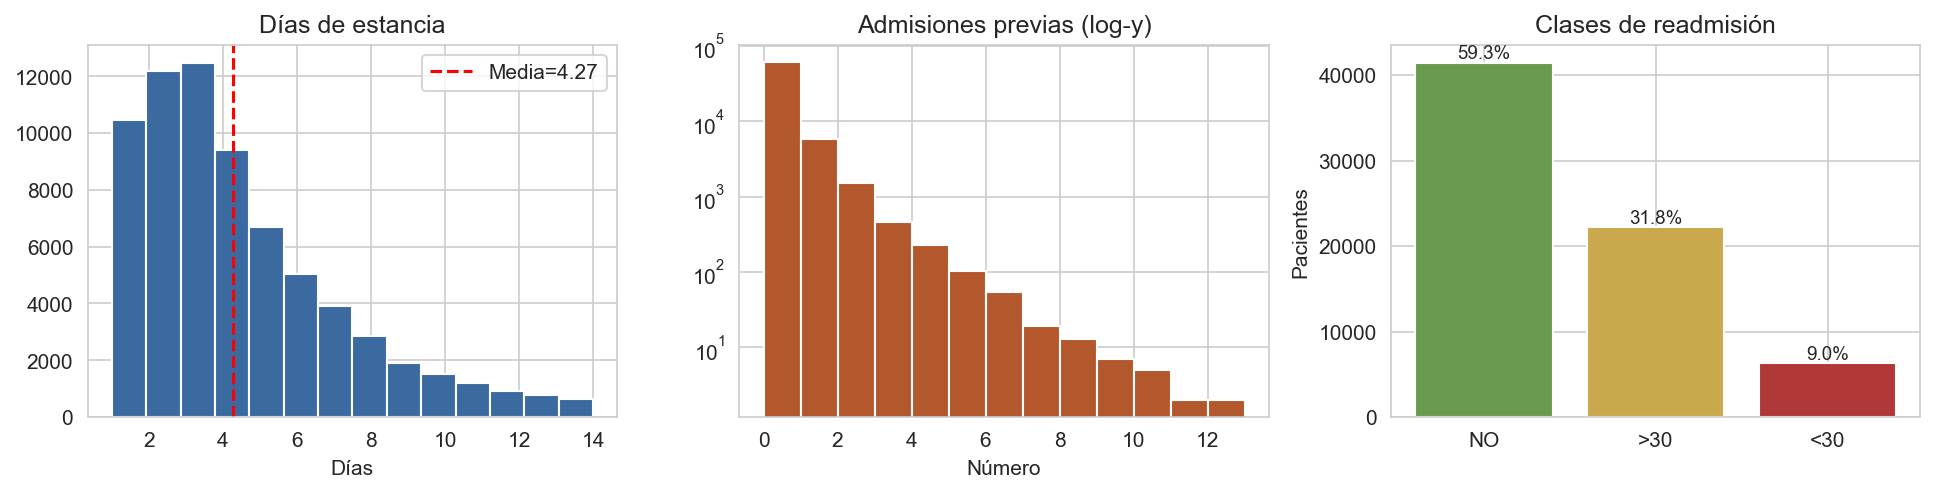
\includegraphics[width=0.95\linewidth]{figuras/fig1_distribuciones.png}
\caption{Distribuciones de las variables respuesta: estancia, admisiones previas y readmisión a 30 días.}
\label{fig:dist}
\end{figure}

La estancia está sesgada a la derecha: la mayoría de los pacientes permanece pocos días, pero algunos se quedan mucho más. La recurrencia tiene muchos ceros y una cola larga. La readmisión a 30 días es un evento poco frecuente.

También se revisó la tasa de readmisión por edad.

\begin{figure}[H]
\centering
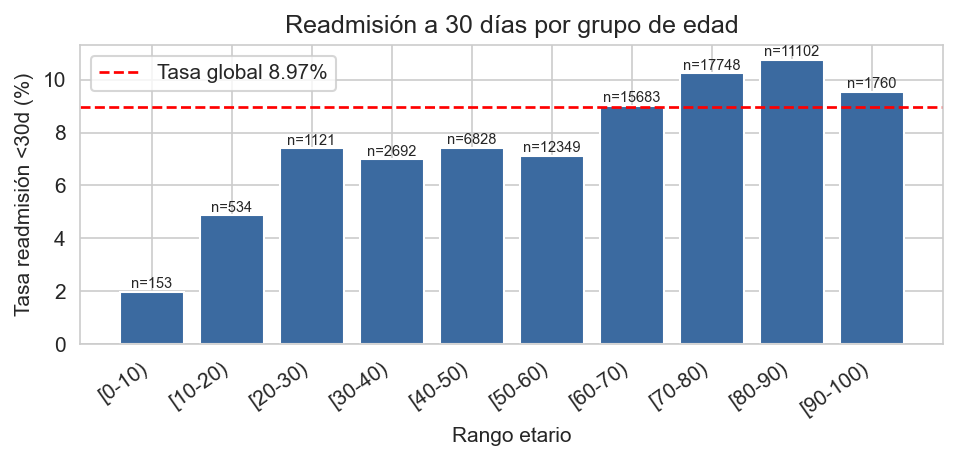
\includegraphics[width=0.85\linewidth]{figuras/fig2_readmit_edad.png}
\caption{Tasa de readmisión a 30 días por grupo de edad.}
\label{fig:edad}
\end{figure}

La tasa no es estrictamente lineal, pero los grupos de mayor edad presentan tasas más altas y estables, lo que es consistente con la mayor comorbilidad y uso del sistema de salud en esos rangos.

Para revisar relaciones entre variables numéricas se usó correlación de Spearman. Se eligió Spearman porque varias variables son asimétricas y no siguen una relación lineal simple.

\begin{figure}[H]
\centering
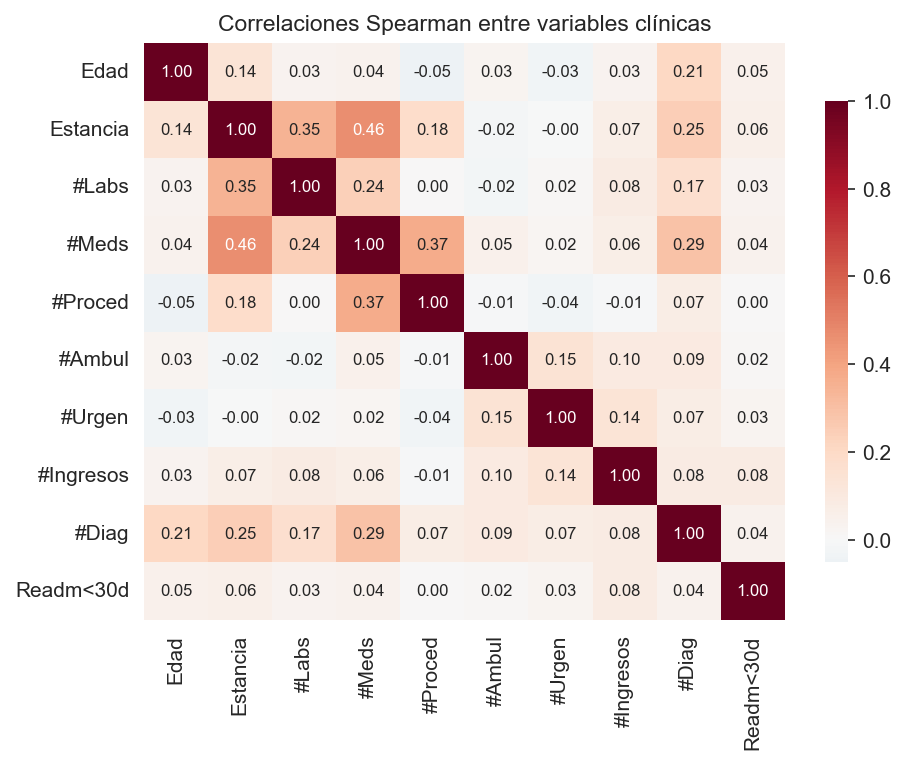
\includegraphics[width=0.72\linewidth]{figuras/fig3_corr_spearman.png}
\caption{Correlación de Spearman entre variables clínicas y de uso hospitalario.}
\label{fig:corr}
\end{figure}

La matriz muestra que las variables de uso previo del hospital se mueven juntas: los pacientes que ya han usado más urgencias, hospitalización o servicios ambulatorios tienden a formar un grupo de mayor carga operativa.

\section{Inferencia estadística}

Después del análisis visual se aplicaron pruebas estadísticas para confirmar si los patrones observados eran razonables.

Se usaron:

\begin{itemize}
    \item Kolmogorov-Smirnov para revisar la forma de la estancia;
    \item Mann-Whitney para comparar estancia entre pacientes readmitidos y no readmitidos;
    \item Chi-cuadrada para revisar asociación entre diagnóstico y readmisión;
    \item Kruskal-Wallis para comparar estancia entre grupos de edad.
\end{itemize}

Los resultados confirman que existen diferencias reales entre los grupos. Aun así, con un tamaño de muestra tan grande casi cualquier diferencia resulta estadísticamente significativa, por lo que el valor del p-valor por sí solo no basta. Por eso se acompañaron las pruebas con tamaños de efecto, que cuantifican la magnitud práctica de cada diferencia (Tabla \ref{tab:effects}).

\begin{table}[H]
\centering
\caption{Pruebas de inferencia y tamaños de efecto correspondientes}
\label{tab:effects}
\begin{tabular}{lcccl}
\toprule
Prueba & Estadístico & p-valor & Efecto & Magnitud \\
\midrule
Mann-Whitney (estancia $\sim$ readmisión) & $U=1.76\times 10^8$ & $1.7\times 10^{-56}$ & Cliff's $\delta = -0.12$ & pequeño \\
Chi$^2$ (diagnóstico $\times$ readmisión) & $\chi^2 = 75.2$ & $1.4\times 10^{-12}$ & V de Cramér $= 0.033$ & trivial \\
Kruskal-Wallis (estancia $\sim$ edad) & $H = 1{,}439$ & $\sim 0$ & $\varepsilon^2 = 0.020$ & pequeño \\
\bottomrule
\end{tabular}
\end{table}

La interpretación es coherente: aunque los tres p-valores son cercanos a cero, las magnitudes de efecto son pequeñas. Es decir, las diferencias son reales pero modestas. Una diferencia de un día en la mediana de estancia es estadísticamente menor pero relevante a escala hospitalaria.

\section{Modelos estadísticos}

\subsection*{Diseño común}

Para los tres modelos se siguió el mismo protocolo: división estratificada del conjunto en entrenamiento (75\,\%) y prueba (25\,\%), con semilla fija para garantizar reproducibilidad. Las variables categóricas se codificaron mediante variables \textit{dummy} con eliminación de la primera categoría para evitar colinealidad. El ajuste se realizó con \texttt{statsmodels}, que permite reportar errores estándar e intervalos de confianza adecuados para inferencia. La elección de cada métrica de evaluación responde a la naturaleza de la variable: AUC y curva ROC para la binaria, AIC para los modelos de conteo y devianza explicada para el modelo Gamma.

\subsection{Readmisión a 30 días}

Para readmisión se usó regresión logística, porque la variable objetivo es binaria: el paciente se readmite en menos de 30 días o no.

El desempeño en el conjunto de prueba fue:

\begin{itemize}
    \item Prevalencia de la clase positiva: 8.97\,\% (clase desbalanceada).
    \item AUC ROC: 0.608.
    \item PR-AUC (precisión promedio): 0.137, frente a una línea base aleatoria de 0.090.
    \item Pseudo \(R^2\) de McFadden: 0.023.
\end{itemize}

Con una prevalencia tan baja, la curva ROC tiende a sobreestimar el desempeño percibido; por eso se reporta también la curva precisión-recall, más informativa cuando la clase positiva es rara (Figura \ref{fig:rocpr}). El AUC obtenido es modesto pero coherente con el rango típico de la literatura cuando se utilizan únicamente variables administrativas y clínicas estructuradas, sin notas médicas ni biomarcadores.

\begin{figure}[H]
\centering
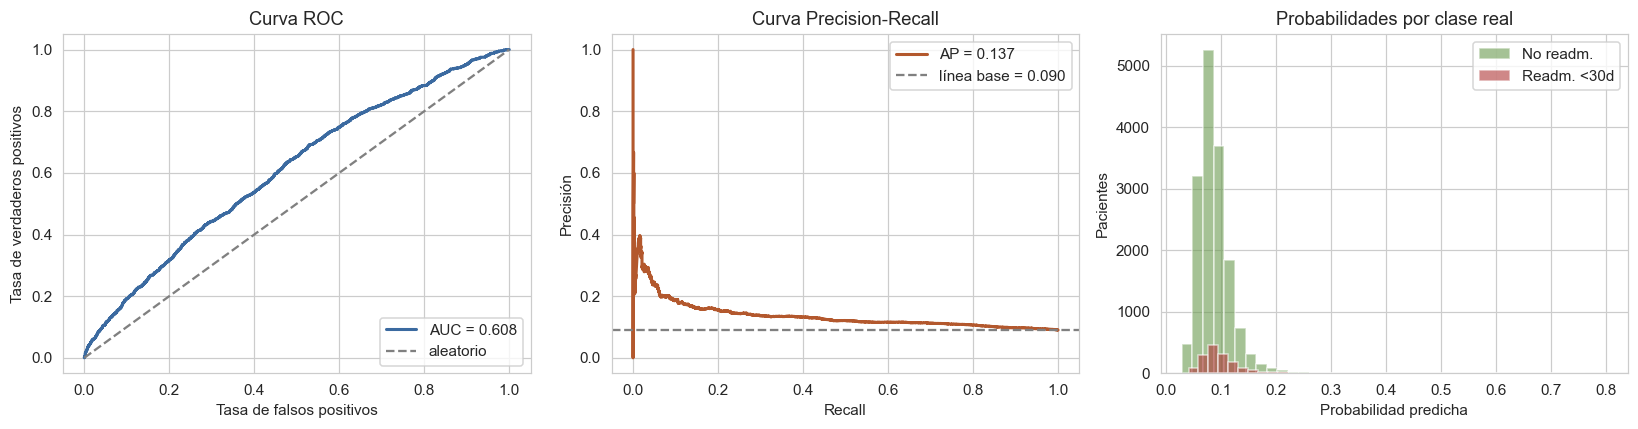
\includegraphics[width=0.95\linewidth]{figuras/fig6_roc_pr_logistica.png}
\caption{Diagnóstico del modelo logístico: curva ROC, curva precisión-recall y distribución de probabilidades predichas por clase real.}
\label{fig:rocpr}
\end{figure}

El modelo no predice de forma exacta, pero sí permite identificar qué factores acompañan al riesgo de readmisión.

\begin{figure}[H]
\centering
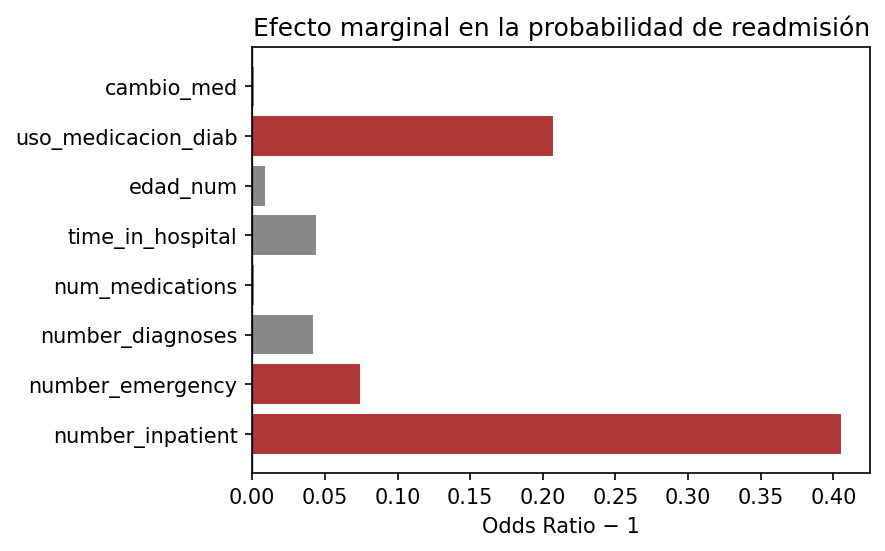
\includegraphics[width=0.78\linewidth]{figuras/fig4_or_logistica.png}
\caption{Efectos principales de la regresión logística expresados como factores multiplicativos sobre la probabilidad de readmisión, con intervalos de confianza al 95\,\%.}
\label{fig:or}
\end{figure}

Los efectos más relevantes (Tabla \ref{tab:or}) fueron:

\begin{table}[H]
\centering
\caption{Factores asociados con la readmisión a 30 días (todos con $p < 0.01$)}
\label{tab:or}
\begin{tabular}{lcc}
\toprule
Variable & Factor multiplicativo & IC 95\,\% \\
\midrule
Admisiones previas (cada una) & 1.40 & [1.36, 1.46] \\
Uso de medicamento para diabetes & 1.21 & [1.11, 1.32] \\
Visitas previas a urgencias & 1.07 & [1.03, 1.12] \\
Días de estancia (cada uno)   & 1.04 & [1.03, 1.06] \\
Número de diagnósticos (cada uno) & 1.04 & [1.02, 1.06] \\
\bottomrule
\end{tabular}
\end{table}

El predictor más importante es el historial de admisiones previas: cada ingreso adicional aumenta la probabilidad de readmisión por un factor cercano a 1.40 (alrededor de 40\,\% más alta que la de un paciente comparable sin ese antecedente). En conjunto, los pacientes con mayor historia de uso hospitalario presentan un mayor riesgo de readmisión temprana.

\subsection{Recurrencia hospitalaria}

La recurrencia se modeló como conteo. Primero se probó Poisson, pero los datos mostraban sobredispersión: la varianza era mayor que la media. Por eso se comparó contra una Binomial Negativa. Los modelos se compararon mediante el AIC (\textit{criterio de información de Akaike}), una medida que combina el ajuste del modelo con una penalización por su complejidad: a menor AIC, mejor balance entre ajuste y parsimonia.

\begin{table}[H]
\centering
\caption{Comparación de modelos para recurrencia hospitalaria}
\begin{tabular}{lccc}
\toprule
Modelo & AIC & Dispersión Pearson & Pseudo \(R^2\) \\
\midrule
Poisson & 73,034.86 & 1.93 & 0.129 \\
Binomial Negativa & 64,529.27 & 1.06 & 0.065 \\
\bottomrule
\end{tabular}
\end{table}

La Binomial Negativa obtuvo un AIC sustancialmente menor ($\Delta\text{AIC} \approx 8{,}688$ a favor de la Binomial Negativa), lo que confirma que la recurrencia presenta sobredispersión (Figura \ref{fig:aic}): un subconjunto de pacientes concentra una fracción desproporcionada del uso hospitalario.

\begin{figure}[H]
\centering
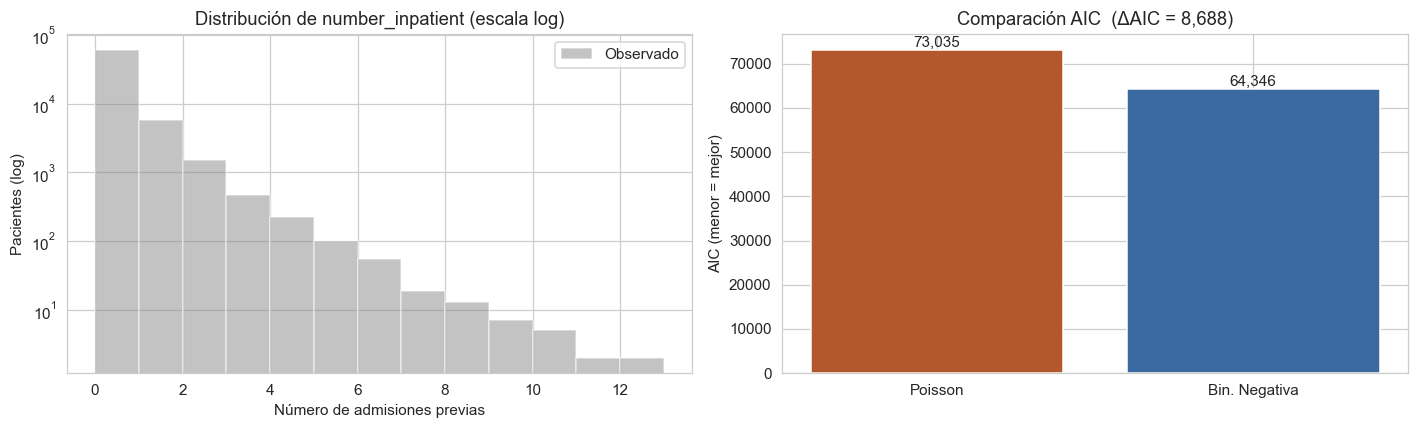
\includegraphics[width=0.92\linewidth]{figuras/fig7_aic_poisson_nb.png}
\caption{Distribución observada de admisiones previas (escala logarítmica) y comparación de AIC entre los modelos Poisson y Binomial Negativa.}
\label{fig:aic}
\end{figure}

Los efectos más fuertes (leídos como \textit{incidence rate ratios}, IRR) fueron las visitas previas a urgencias (IRR $= 1.77$), el uso de medicamento para diabetes (IRR $= 1.24$) y las visitas ambulatorias previas (IRR $= 1.13$). Una visita adicional a urgencias multiplica el conteo esperado de admisiones por 1.77; este resultado ofrece un criterio operativo claro para identificar estos pacientes antes del alta.

\subsection{Duración de la estancia}

Para la duración de estancia se usó un modelo Gamma con enlace logarítmico. La razón es sencilla: los días de estancia son positivos y tienen sesgo a la derecha.

\begin{figure}[H]
\centering
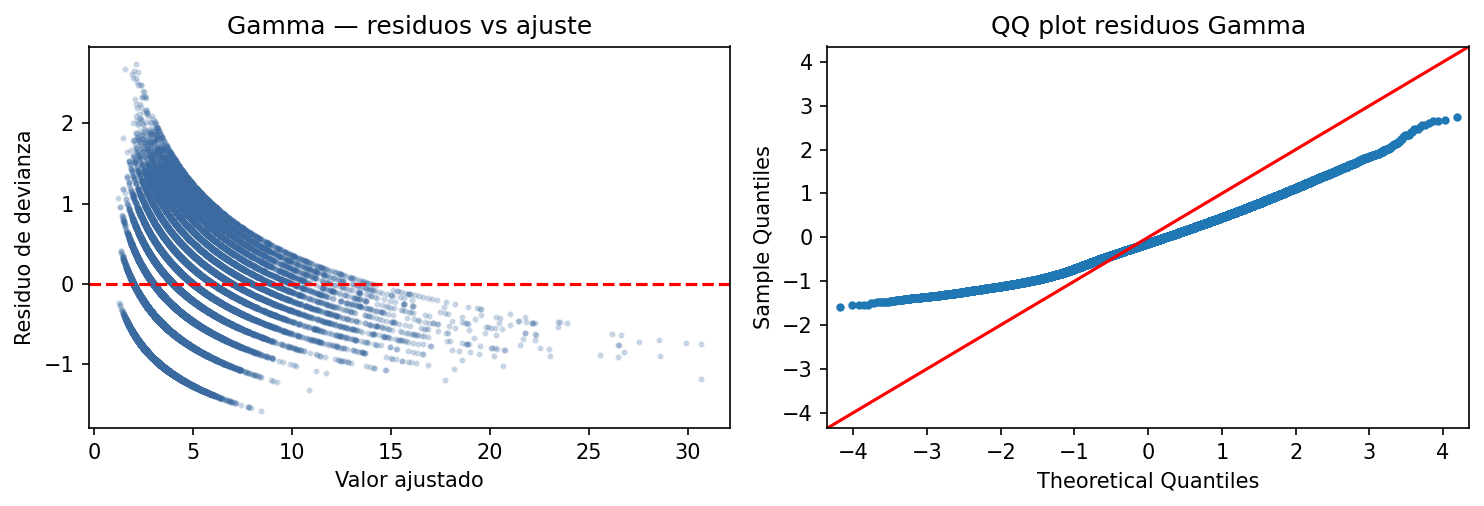
\includegraphics[width=0.92\linewidth]{figuras/fig5_diag_gamma.png}
\caption{Diagnóstico del modelo Gamma para duración de estancia.}
\label{fig:gamma}
\end{figure}

El modelo Gamma alcanzó un pseudo $R^2$ basado en devianza de 0.28, un valor satisfactorio para datos clínicos administrativos. Tomando como referencia la categoría diagnóstica circulatoria (eliminada como base por la codificación con \textit{drop\_first}), las estancias en categorías como ``Otros'' (factor 1.34), Neoplasmas (1.29) y Diabetes (1.24) tienden a ser más prolongadas. Cada diagnóstico adicional incrementa la estancia esperada en aproximadamente 3\,\%, y cada admisión previa en alrededor de 3\,\%. En conjunto, la complejidad clínica del paciente es el factor principal que determina la duración esperada de la hospitalización.

\section{Recomendaciones}

Los resultados se pueden traducir en tres recomendaciones:

\begin{enumerate}
    \item Crear un programa de seguimiento al alta para pacientes con mayor uso previo del hospital.
    \item Usar visitas previas a urgencias e ingresos previos como señales tempranas de recurrencia.
    \item Considerar diagnóstico y complejidad clínica para planear camas y recursos.
\end{enumerate}

La recomendación principal es priorizar a los pacientes con mayor complejidad clínica y mayor uso previo del sistema. Dado que el riesgo no es homogéneo, una asignación diferenciada de recursos resulta más eficiente desde el punto de vista operativo.

\section{Limitaciones}

El análisis describe asociaciones, no relaciones causales. Adicionalmente, el dataset es de naturaleza administrativa, contiene faltantes relevantes y corresponde a hospitales de Estados Unidos entre 1999 y 2008. Las conclusiones específicas deben interpretarse como una guía contextual, no como una regla generalizable.

Trabajar con un único registro por paciente mejora la independencia de las observaciones, pero reduce el tamaño efectivo de la muestra y descarta información sobre la trayectoria de cada paciente a lo largo del tiempo. Esto implica que el análisis describe el riesgo en una única visita, pero no captura cómo evoluciona ese riesgo con sucesivas admisiones. Una extensión natural sería utilizar modelos longitudinales o de efectos mixtos, que permiten incluir todas las admisiones de un mismo paciente reconociendo que esas observaciones están correlacionadas entre sí, en lugar de tratarlas como si fueran independientes.

\section{Conclusión}

La readmisión, la recurrencia y la duración de la estancia comparten señales comunes de complejidad clínica y uso previo del sistema, aunque no constituyen el mismo fenómeno. Por ello se utilizaron herramientas distintas: regresión logística para readmisión, modelos de conteo para recurrencia y un modelo Gamma para la estancia.

La conclusión central es que los pacientes con mayor historia de uso hospitalario y mayor complejidad clínica concentran buena parte del riesgo operativo. Su identificación temprana puede contribuir a reducir readmisiones, optimizar la planeación de camas y mejorar el seguimiento posterior al alta.

\section*{Referencias}

\begin{enumerate}[label={[\arabic*]}]
    \item Strack, B., DeShazo, J. P., Gennings, C., Olmo, J. L., Ventura, S., Cios, K. J., y Clore, J. N. (2014). \textit{Impact of HbA1c measurement on hospital readmission rates: analysis of 70,000 clinical database patient records}. BioMed Research International, 2014, 781670.
    \item Cameron, A. C. y Trivedi, P. K. (2013). \textit{Regression Analysis of Count Data}, 2.\textsuperscript{a} ed. Cambridge University Press.
    \item McCullagh, P. y Nelder, J. A. (1989). \textit{Generalized Linear Models}, 2.\textsuperscript{a} ed. Chapman \& Hall/CRC.
    \item Agency for Healthcare Research and Quality (AHRQ). \textit{Clinical Classifications Software (CCS) for ICD-9-CM}. Disponible en: \texttt{hcup-us.ahrq.gov}.
    \item Akaike, H. (1974). \textit{A new look at the statistical model identification}. IEEE Transactions on Automatic Control, 19(6), 716--723.
    \item Seabold, S. y Perktold, J. (2010). \textit{Statsmodels: Econometric and statistical modeling with Python}. Proceedings of the 9th Python in Science Conference.
\end{enumerate}

\end{document}
